\ofsubsection{Ivalice Worldbook}
%
\ofquote{"Names don't matter. What's important is how you live your life."}{Ramza Belouve}\\\\
%
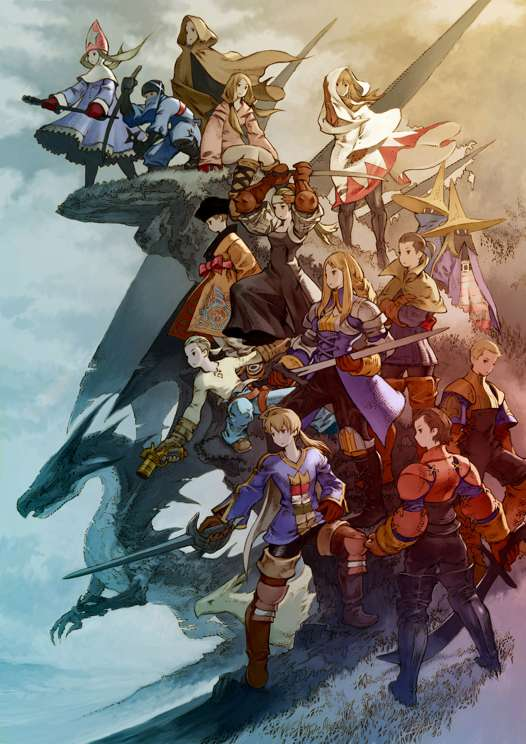
\includegraphics[width=\columnwidth]{./art/worldbook/everyone.jpg}
%
\ofrow
%
The \accf{Ivalice Worldbook} is a comprehensive document about the setting of the Final Fantasy Tactics video game.
It includes many details about its history and geography to help you create your own adventures in the same world.
This supplement is an updated version of the original version written by Bruno Carvalho, Paul (Papa Quackers) and Hywel Williams in 2017 which included rules for the Final Fantasy Role Playing Game 4th Edition~(\accf{FFPRG~4e}) system.
This version instead includes optional rules for Omega~Fantasy at its end.
Nevertheless, the vast majority of the content and ideas presented in this worldbook are system agnostic and thus applicable to other tabletop RPGs.
%
\ofpar
%
\accf{Final Fantasy Tactics}~(FFT) is a spin-off title in the main Final Fantasy series. 
Unlike most spin-offs, however, it has managed to be a great game on its own, having received universal acclaim upon its release, and critical opinion of the game has improved further over time. 
It is the first game of the Final Fantasy Tactics series and was released in Japan in June 1997 and in the United States in January 1998. 
The game combines thematic elements of the Final Fantasy video game series with a game engine and battle system unlike those previously seen in the franchise. 
In contrast to other 32-bit era Final Fantasy titles, Final Fantasy Tactics uses a 3D, isometric, rotatable playing field, with bitmap sprite characters.
For many Final Fantasy players, this represented their first foray into the Strategy RPG genre, with its own quirks and conventions established by several other games that came before, like Shining Force, the Langrisser series or Tactics Ogre. 
For this reason, and to celebrate the 20th anniversary of the original Japan release of this cult classic, this worldbook was born.
%
\vfill
%
Final Fantasy Tactics uses a three-dimensional isometric battle grid. 
This difference in functionality led to a game type that was more akin to chess than the traditional back and forth linear combat of previous Final Fantasy games. 
Instead of having six characters that were all-essential to the plot, and joined your party over a period, you had a singular main character that would occasionally be joined by story important characters that would depart and rejoin you when the plot demanded they do so. 
The bulk of your adventuring party was usually made up of interchangeable, nondescript characters whose appearance shifted radically depending on what \accf{job class} they were.
The progression of job classes in this system is quite similar to that of older Final Fantasy games, in that there were several job classes to choose from, but fundamentally different in how certain
job classes were unlocked. 
Instead of obtaining crystals that granted certain job classes automatically, you were given two starting job classes and expanded upon them. 
Your job progress reveals others, and if you took multiple levels in multiple jobs, your amalgamated experience in those two jobs might reveal another job class that was unique. 
This system involved a lot of job class switching and of course, a small amount of class mapping to determine which job classes unlocked another.
%
\vfill
%
\ofquote{"The best ways, don't always lead to the best results."\\}{Delita Hyral}\\\\
%
The story of Final Fantasy Tactics revolves around the aftermath of \accf{The 50 Year War}. 
The kingdom of \accf{Ivalice} is rife with political and economic discrepancies between the upper and lower class. 
This problem is compounded by the recent death of the king, whose only heir is an infant, and the need for a regent to rule in his place. 
The people are stuck between Prince Goltana, and Prince Large, known as the Black and White Lion respectively.
This leads into the main plot of the game, known as \accf{The Lion War}, in which you take on the role of \accf{Ramza Beoulve}. 
As the name implies, The Lion Wars were conflicts between the two princes in their attempt to become the ruling regent. 
Ramza is a young noble who takes part in many exploits of the war, discovers hidden corruption and machinations within the most powerful church in the lands, and comes to understand the plight of the common peoples. 
He was a decisive factor in the resolution of the war but was actively erased from history.
%
%
%
\clearpage
%
\ofsubsubsection{History}
%
\accf{The Beginning (10000 B.C. -- 2000 B.C.)}\\
During this period of time, estimated from 10000 to 2000 B.C. on the Ajorian Calendar, the majority of humankind lived on the southwestern coast of what years later would become Kaladis. 
Most of the people of these times were simply tribes of hunter-gatherers. 
As the age neared its close, however, metallurgy was developed as well as basic magic study. 
Unfortunately, there are extremely few records from this period, partly in thanks to a lack of a written language, which was first developed during the age of the Ronan Empire, although there are some rare ruins left behind that have been found in remote parts of Kaladis.
During this period, the countries that would later become Kaladis and Mizuno were first settled. Ivalice, Romanda, and Ordalia were first settled during the Ronan Empire.
%
\ofpar
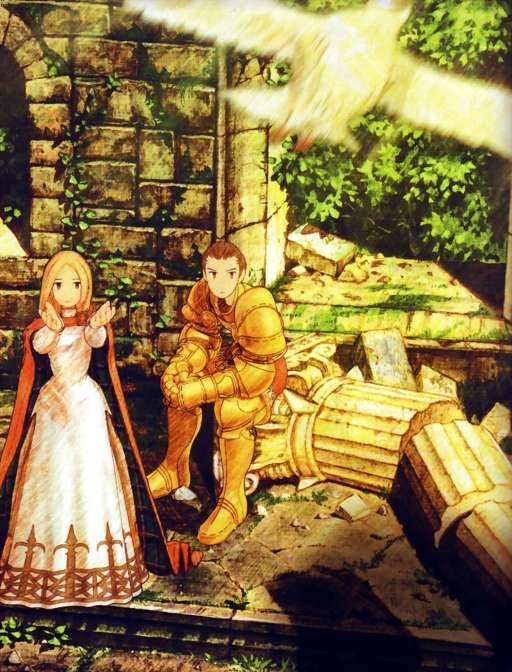
\includegraphics[width=\columnwidth]{./art/worldbook/ovelia.jpg}
\ofpar
%
\accf{The Ronan Empire (2000 B.C. -- 700 B.C.)}\\
History dates the first true civilization as the Ronan Empire; an empire that grew from a humble farm village near Zeltenia to a huge empire that spanned most of what would become Ivalice and parts of Romanda and Ordalia near its end, roughly estimated between 700 and 600 B.C.. 
Not much is known about this mysterious empire save that it excelled at the use of magic even compared to the level used by the most powerful of today's magicians. 
Even more mysterious is what caused its downfall. 
The Ronan Palace, the center of the empire, was up until its discovery during the Lion Wars a myth in and of itself. 
Several important ruins originated from this era including Matoya's cave, the Tower of Babel, Mirage Tower, and of course the \accf{Ronan Palace}. 
The Ronan Empire was the first country to develop a written language with Mizuno soon following within its own language known as Nihonjin.
%
\ofpar
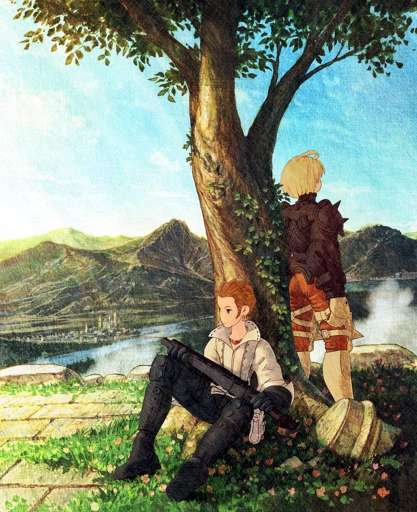
\includegraphics[width=\columnwidth]{./art/worldbook/tree.jpg}
\ofrow
%
\accf{The Age of Myth (700 B.C. -- 50 B.C.)}\\
Following the downfall of the Ronan Empire, the territories splintered into four separate countries: Melmond, the Baron Kingdom, the Kushuka Kingdom, and the Palamecian Empire. 
Like the Ronan Empire, these four nations covered Ivalice and began making inroads into the areas that would become Romanda and Ordalia in later years. 
This period is largely known as the age of myth in part due to the amount of fantastic ruins that were left behind as well as the level of technology developed.
\accf{Baron Kingdom} was a kingdom whose military might rivaled many of the other nations during the age of myth. 
Baron supported a large number of elite knights as well as a well-known navy of airships. 
Baron covered much of what would become Gallione, Fovoham, and western Lesalia.  
Compared to its neighbors, the \accf{Kushuka Kingdom} was a center of trade where traders from other countries would come to sell their wares. 
Unfortunately, for the country itself, its nobility ruled with harsh hand with little concern for their people.
After years of abusing the coffers of their nation, the royal family was dethroned by a huge revolution. 
On a modern map, Kushuka would occupy much of central Lesalia and most of Zeltenia.
Like its neighbors, the \accf{Palamecian Empire} had a specialty, namely technology. 
It was the first to develop airships and maintained a fleet that was a fair equivalent of Baron's navy. 
In addition to its airships, Palamecia also first developed guns that used magical ammunition as well as its "war golems", powerful robots that were used as first line soldiers and guards. 
The empire covered what would become Lionel. 
Many historians believe that its capital is deep below Goug Machine City. 
Palamecia was also the first to develop steam-powered devices and were the first to develop the science of magitek, which involves the fusing of magic and machine.
\accf{Melmond} was a secluded nation far to the east in what would later become southern Ordalia. 
More than other countries, Melmond embraced the study of magic in full and supported many academies dedicated to teaching the arcane arts to interested students. 
Other studies such as history, philosophy, and literature were also popular among Melmond people. 
Unfortunately, Melmond was considered by many of its neighboring countries to be working with the forces of Lucavi because of their magical might.
Like the Ronan Empire before them, all four kingdoms of the age of myth were destroyed by unknown circumstances. 
The \accf{Zodiac Brave Story} first emerged during this era. 
For those that do not know it, the Zodiac Brave Story is the tale of an evil king who called on the powers of Lucavi, around the year 500~B.C..
Lucavi killed the king and caused great havoc throughout the world. 
In the end, a small group of 12 heroes banded together and used the sacred zodiac stones to become the Zodiac Braves. 
The Zodiac Braves were able to defeat Lucavi and supposedly restored order. 
Following the defeat of Lucavi, the \accf{Holy Ydoran Empire} was founded, emerging from the ruins of the old Baron Kingdom.
The empire waged several wars, eventually defeating and conquering both Palamecia and Melmond.
%
\vfill
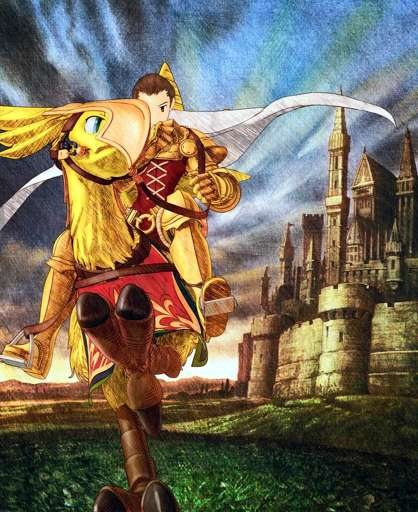
\includegraphics[width=\columnwidth]{./art/worldbook/delita2.jpg} 	
%
\newpage
%
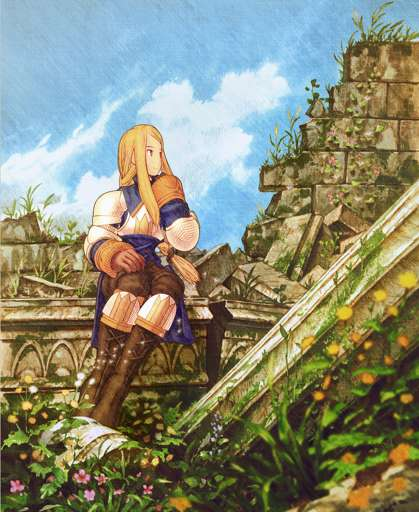
\includegraphics[width=\columnwidth]{./art/worldbook/agrias.jpg}
\ofpar
%
\accf{The Life \& Death of St.~Ajora (50 B.C. -- 1 B.C.)}\\
The Ajorian Calendar begins its first year with the death of \accf{St.~Ajora} and the beginning of the \accf{Cataclysm}. 
By the time Ajora Glabados came, three of the four kingdoms of the age of myth had been conquered by the Holy Ydoran Empire, and the Kushuka Kingdom was the only other state to resist the power of its neighbor. 
The lands that once were Melmond laid abandoned and desolate, as refugees from the Jihads that would follow the rise of the Glabados Church would only resettle them several centuries later.
When Ajora Glabados was young, one day he sprang up, walked to a well, and prophesized that "soon, a calamity will befall this land. 
I am now sealing this well, and no one can drink from it." Several days later, the "Black Death" plagued Zeltenia. 
The people who drank from the contaminated well water fell ill and died one after another.
However, only the families that believed Saint Ajora's words survived and did not fall to disease. 
Since then, Saint Ajora became worshipped as "The Miracle Child" or "The Son of God".
Soon after these events, word of a new messiah spread, who would lead Ivalice out of the chaos born from years of war. 
By the time Ajora had reached 18 years old, he had already gained a devoted community of followers. 
Much like in earlier years, another ambitious king attempted to summon Lucavi. 
The emperor had created an army of immense size in the hopes of securing all of Ivalice under the Holy Ydoran Empire’s control. 
Once again, a new group of Zodiac Braves was created united by St.~Ajora to defeat the new Lucavi.
Despite his growing widespread fame, Ajora had made many enemies. 
The Holy Ydoran Empire feared Saint Ajora's rise to power; they feared his preaching of the coming of God. 
The \accf{Clergy of the Pharism} faith was the predominant religion and even though they had great influence, the clergy feared Saint Ajora's power. 
The conclusion is obvious.
Saint Ajora was captured with a secret tip from Germonik, Ajora's 13th Apostle. 
Saint Ajora was executed at the Golgollada execution site. 
However, Saint Ajora was the "Son of God". 
God's anger struck at Pheisias, and the Cataclysm began, a series of seismic and volcanic events that shocked the world for the next 25 years.
The Cataclysm is often assumed to be the cause behind the loss of Ivalice's most advanced technologies, though the game never outright states this. 
It also destroyed at least two races, the "winged ones" (possibly the aegyl), the moogles (as told in the Siedge Weald) and the Clockwork City of Goug, and if the Ivalician myth is true, threatened humanity, leading some to believe it is responsible for the disappearance of the non-human races from Ivalice. 
The sinking of Mullonde, involving the drowning of an entire state of the Ivalician peninsula, also relates to it. 
The Cataclysm created the Floating Continent, and destroyed Eureka and of the Fortress of Trials. 
According to legend, the Hero-King Mesa saved humanity from its effects.
%
\ofpar
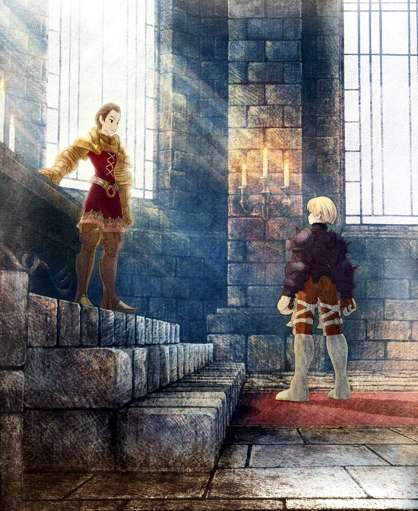
\includegraphics[width=\columnwidth]{./art/worldbook/delita.jpg}
\ofpar
%
\accf{Rise of Gloabados Church (25 A.C -- 1112 A.C.)}\\
Following the death of Saint Ajora, his remaining apostles established a new church under his name: the \accf{Glabados Church}, using its namesake's exploits.
Soon after its establishment, it was able to cooperate with warring nations that sprung after the cataclysm and subsequent collapse of the Holy Ydoran Empire on a working peace treaty that set up the \accf{Atkasha} family as the rulers of Ivalice. 
As part of the peace treaty, Limberry was assimilated into Ivalice. 
Despite the end of pen warfare among the remaining nations, a new cold war developed between the remaining followers of the Fara Clergy and the newly formed Glabados Church.
As Pharism was weakened thanks to the tragedy that led to the destruction of the Ydoran Empire, the Glabados church had no trouble forcing the Phara Clergy and its remaining followers from Ivalice. 
The remaining Phara followers would, slowly over the next 300 years, help create the nation of Ordalia to the east.
The Glabados Church during the first 1000 years of its existence was very powerful, to say the least.
Thanks to its iron handed fist, it helped create several different splinter factions of the Glabados religion, including the Argades church, which would later become the official religion of the Romanda Empire.
%
\ofpar
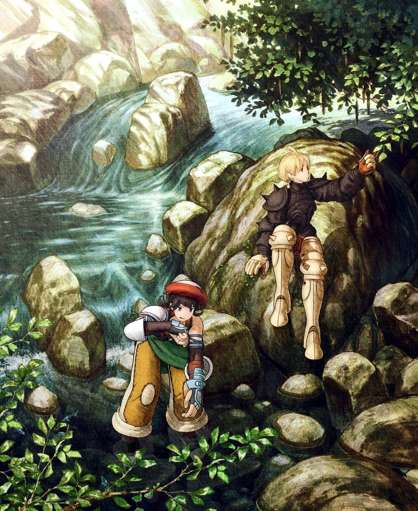
\includegraphics[width=\columnwidth]{./art/worldbook/luso.jpg}
\ofpar
%
\accf{The Fifty Years War (1113 A.C -- 1163 A.C.)}\\
By 1113, King Denamda II ruled Ivalice, while King Devanne III ruled its neighboring kingdom, Ordalia. 
Three knightly orders defended Ivalice: the Order of the Northern Sky Knights, led by Ramza's father, \accf{Barbaneth Beoulve}, the Order of the Southern Sky Knights led by \accf{Cidolfus Orlandeau}, and the Order of the Eastern Sky, under the leadership of \accf{Goffard Gaffgarion}. 
Gustav Margriff and \accf{Wiegraf Folles} served within the Order of the Northern Sky.
Strife erupted at Zelmonia, a once independent province near to Ivalice's border and now under Ordalian rule. 
About a century ago, Ordalia invaded and assimilated Zelmonia. 
Ivalice had secretly provided means to weaken Ordalia; however, the Zelmonian nobles decided to petition for King Denamda's direct intervention. 
King Devanne III died without naming a successor. 
His cousin Varoi VI was named as successor, but King Denamda II proclaimed himself as rightful heir, being Devanne's uncle, and declared war against Ordalia.
King Denamda II led the Ivalice army towards the Ordalian capital of Viura. 
On their way, knights of the three Orders fought valiantly, winning battle after battle.
As they were reaching the Ordalian border, King Denamda II fell ill and died soon after, never able to return to his kingdom. The Ivalician army became lost and confused due to their leader's death and Ordalia used that as an opportunity to strengthen its army and defend the borders. 
%
\vspace*{0.5cm}
%
\begin{center}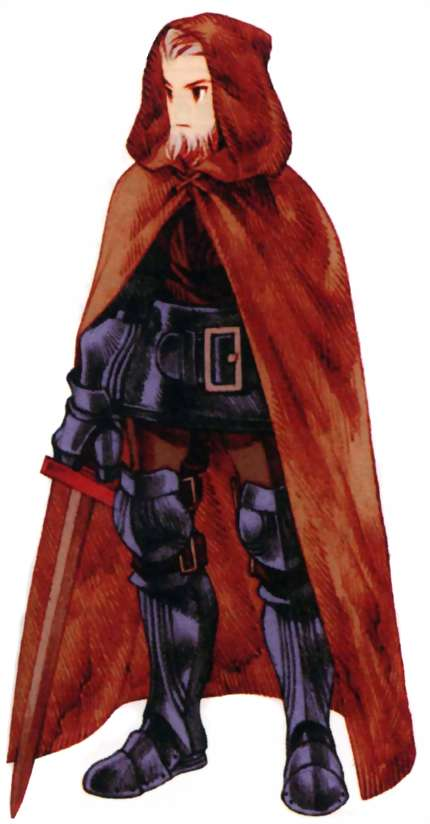
\includegraphics[width=0.65\columnwidth]{./art/worldbook/cid.jpg}\end{center}
%
\vspace*{0.5cm}
%
The war raged fiercely, reaching a stalemate. 
A successor to Denamda II, Denamda III, was hastily enthroned to replace his father.
During the stalemate, Romanda's armies crossed the Rhana Strait in an invasion upon Ivalice. 
Romanda was a military nation ruled by a blood relative of King Varoi VI. 
King Denamda IV and his Ivalician army held off the invasion through the aid of Fovea’s ruler, Grand Duke Gerrith Barrington, and his assassination squad Khamja.
After three years of fighting, Romanda retreated. 
King Denamda IV was a fearless warrior who personally led his armies in battles against the combined forces of Romanda and Ordalia. 
The outbreak of Black Death within Romanda also led to their retreat.
With Romanda's retreat, Ivalice continued with the war against Ordalia.
Denamda IV died suddenly, believed to be assassinated. 
He was succeeded by King Ondoria Atkascha III, although the king was a weak-willed man and unfit to rule, and all his decisions being made by \accf{Queen Louveria}.
Ordalia's ruler Varoi VI also died, and was replaced by Prince Lennard. 
Due to Ondoria's weakness, Ordallia forced Ivalice to cease fighting.
The last battle between Ivalice and Ordallia took place in Zeltennia, and though the Knights of the Orders fought bravely, Ordallia won and occupied the province. 
Ivalice and Ordallia agreed to a mutual peace treaty, though whispers persist that in reality, Ivalice had surrendered.
After the Fifty Years' War, Ivalice suffered a great loss as the people harbored ill feelings and dissatisfaction to the nobles and the royal family who placed them in the meaningless war. 
Farmers staged riots and revolted, and many turned banners to join the \accf{Corpse Brigade}.
Ivalice's economy suffered, as payments could not be made to the knights who had fought in the war due to the spending on weapons and defenses. 
Many were discharged from the army, and with less food and little money, there was high unemployment and disloyalty to the ruling factions grew.
King Ondoria's two sons died, and the king adopted his younger sister, \accf{Princess Ovelia}, as his daughter. 
Soon after, Queen Louveria gave birth to Prince Orinus, causing a conflict over who should become King Ondoria's successor, setting the stage for the War of the Lions.
Rumors spread of King Ondoria's failing health. 
Since his collapse during Prince Orinus' birthday celebration, it became obvious that he was on the brink of death. 
His advisers, the Board of Chamberlains, delivered news that the king was getting better, but the people knew the truth. Soon rumors surfaced that Queen Louveria and other nobles had argued over his successor.
Goffard Gaffgarion was dismissed from the Eastern Sky, and Gustav from the Northern Sky, both on charges of misconduct during the war. 
Gaffgarion turned to the life of a mercenary, claiming allegiance to the highest bidder.
%
\vfill
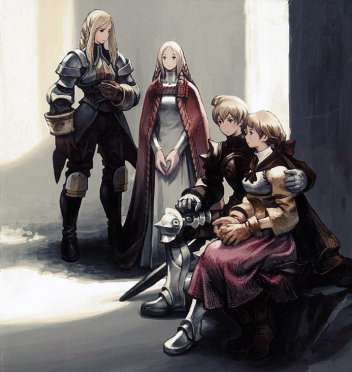
\includegraphics[width=\columnwidth]{./art/worldbook/belouve.jpg}
%
\clearpage
%
\accf{The War of the Lions (1164 A.C -- 1166 A.C.)}\\
The War of the Lions was fought between the Order of the Northern Sky Knights of \accf{Duke Larg} under the banner of the White Lion, and the Order of the Southern Sky Knights of \accf{Duke Goltanna} under the banner of the Black Lion. 
King Ondoria Atkascha III died due to the Black Death and his heir, Prince Orinus, was only two years old. 
A regent was sought to rule in the prince's place, and both dukes who were decorated generals in the Fifty Years' War were nominated as regent.
One of the main reasons behind the War is the rift between Queen Louveria and the nobles of Ivalice. 
Queen Louveria was regarded as a power-mad queen who desired her offspring on the throne so that she may rule the kingdom. 
The Council of Nobles, out to stop her from asserting influence onto the kingdom, appointed Duke Goltanna as their preferred candidate for the regency.
%
\ofpar
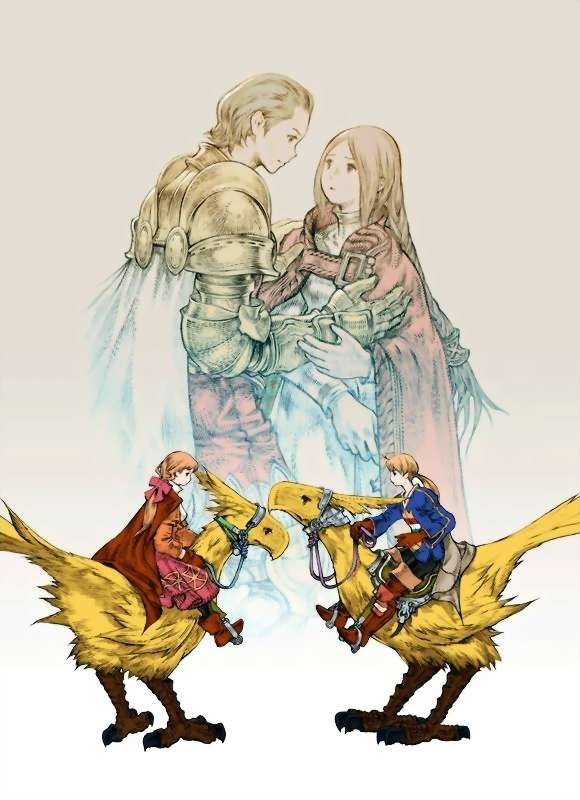
\includegraphics[width=\columnwidth]{./art/worldbook/cover.jpg}
\ofpar
%
The first major battle of the War of the Lions, the Battle of Lesalia Plain, was a massive assault of Chocobo Knights from Gallionne on the plains south of the Royal City of Lesalia, where the royal palace is built. 
The Southern Sky was driven out of the city and forced to their strongholds at Fort Besselat and Limberry Castle. 
The victory lead to Southern plans mostly revolving around an attack on Lesalia, by sending an army led by Cidolfus Orlandeau to take the city, though it was driven away.
Further Southern attempts to attack Lesalia culminated in the Battle of Groffovia, fought on the plains between Limberry, which was generally pro-Southern, and Lesalia proper. 
The battle was inconclusive, but within three months casualties reached 40,000, sapping what little public support the war had.
Around this time, Queen Louveria and Chancellor Glevanne were accused of abducting Princess Ovelia to allow for Duke Larg's ascendancy to the throne. In addition, famine overtook Zeltennia, Limberry, Galionne and Fovoham due to a drought, causing mass starvation among civilians.
The losses sustained by the Southern Sky are worsened by the Battle of the Fusse Plains, in which Marquis Elmdore was killed by a stray arrow. 
He was possessed by the Lucavi \accf{Zalera}, and fought for the Knights Templar at the Battle of Riovanes Castle.
Despite the death of countless soldiers, the war reached a stalemate.
%
\ofpar
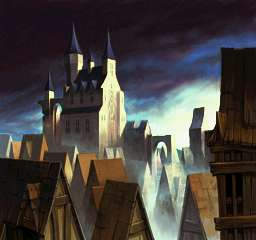
\includegraphics[width=\columnwidth]{./art/worldbook/riovanes.jpg}
\ofpar
% 
The Northern Sky planned to make an all-or-nothing attack at Fort Besselat, planning to take it and use it as a base from which they could wage total war against Southern food supply.
The War's decisive battle was the Battle of Fort Besselat, in which Ramza Beoulve intervened by opening the garrison's sluice, bringing the battle to an indecisive halt. 
Barich Fendsor, one of the Knights Templar, released Mossfungus poison into the air, severely weakening both sides. 
In the confusion, both Dukes were murdered by their respective traitors, Larg by \accf{Dycedarg Beoulve} and Goltanna by \accf{Delita Heiral}. 
As originally planned, the Church offered mediators. 
Despite the loss of both Order's leaders, their armies were still strong and refused the idea. 
This may be because of Ramza's intervention, whereas without it, both sides would have suffered major losses if the sluice were not opened.
Ramza Beoulve traveled with his companions to Orbonne Monastery to stop the Knights Templar and the Lucavi's plot for \accf{Ultima's resurrection}. 
Killing the Church's forces that dared to stop them, they are teleported to the Airship Graveyard beneath the Necropolis of Mullonde and destroyed Ultima, the High Seraph, who wished to destroy Ivalice. 
Their own fate after that is a mystery.
The war finally ended with the two sides crippled. 
With the two dukes killed, Queen Louveria imprisoned in Fort Besselat, High Confessor Funebris murdered, Dycedarg slain, and Orlandeau missing and believed dead, Delita Heiral exploited the situation by claiming that he rescued Princess Ovelia, marrying her to become King of all Ivalice.
The Church of Glabados engineered the War so that it may take the center stage after both sides were weakened due to exhaustion. 
The High Confessor Marcel Funebris, wishing for the Church to gain power over the land, secretly supported both sides and assisted in their plots for the throne. 
The Church planned to destroy the two Lions from the inside and used the Zodiac Stones to strengthen the Church's military power.
%
\ofpar
%
\ofquote{"Your actions have meaning only if they hold true to your ideals."}{Ramza Belouve}\\
%
\begin{center}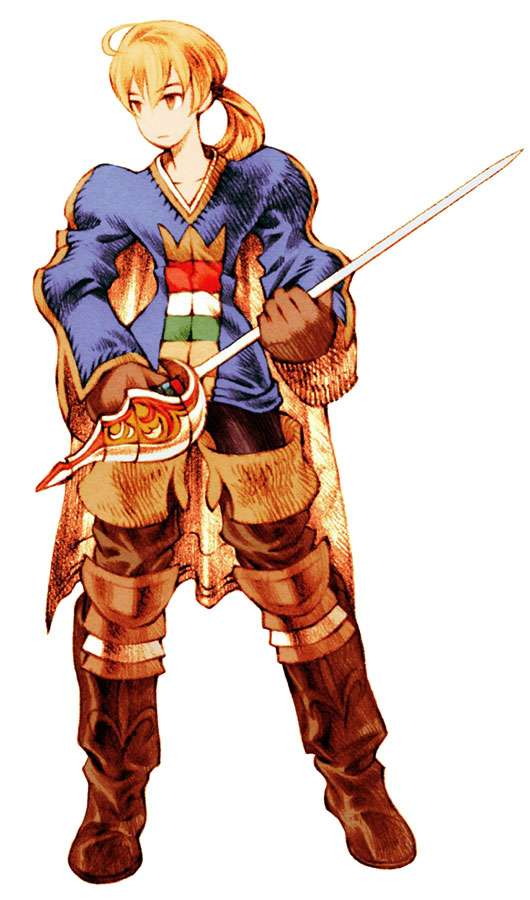
\includegraphics[width=0.85\columnwidth]{./art/worldbook/ramza.jpg}\end{center}
%
%
\accf{The Glabados Schism (1167 A.C. -- 1250 A.C.)}\\
By 1171, the Glabados Church executed \accf{Orran Durai} as a traitor after writing the Durai Papers. 
This caused unrest among several ordained priests, and one of them, Karling Nox, initiated a movement in Limberry which called for reformation within the Church, seeking, in his words, a “return to St.~Ajora’s true ways”. 
This rippled through Ordalia and several of the eastern provinces of Ivalice, and after the Church declared Nox’s status as a heretic, the priest started to gather a sizable following. 
Sensing the opportunity to seize lands and riches from the church, several barons and counts declared their conversion to this new interpretation of Ajoran faith, and gave shelter to the new converts.
Weakened by the events of the Lion War, Glabados was unable to prevent the rise of the self-proclaimed Ajorans, and this religious divide kept growing for the next 80 years. In contrast, the Heiral dynasty's rule proved to be quite unsuccessful in keeping the power centralized, and had to make several concessions to the nobility to maintain its position as the Ivalice King.
These concessions increased the decentralization of the kingdom, empowering the local lords.
By 1240, the religious tensions had turned into violence, with hostilities between Glabados and Ajoran followers leading to several small-scale skirmishes, and culminating with the 1243 massacre of Yardrow, where an angry mob killed a congregation of 500 Ajoran faithful during a religious ritual. 
This sprung several mutual defense treaties between nobles, creating both the \accf{Glabados League}, led by the Grand Duke Rudolph Barrington of Fovoham, and the \accf{Ajoran League}, led by Marquis Henry Elmdore of Limberry. 
The creation of the two leagues only further increased the tension, but for the next seven years, peace reigned inside Ivalice.
In 1250, following a severe disease, king Luther Heiral went into a comatose state. 
His nephew, Paul Heiral, who was a fervorous devout of the Glabados faith, was designated as Regent. 
Fearing to be persecuted by its religious beliefs, the Ajoran League voted for a preemptive war against the Regent, intending to replace him with another noble who is more sympathetic with the Ajoran faith. 
In response, the Glabados League rallied their troops and this plunged Ivalice into civil war.
%
\vfill
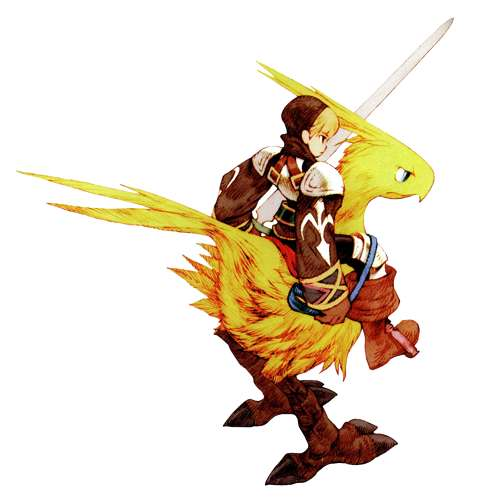
\includegraphics[width=\columnwidth]{./art/worldbook/chocoborider.jpg}
%
\clearpage
%
\ofsubsubsection{Timeline}
%
\newcommand{\nlwb}{\vspace{0.2cm}\\}
%
\oftablewide{p{0.3\columnwidth} p{1.7\columnwidth}}
{\accf{Year} & \accf{Important Events}}
{
	& \\
	< 2000 B.C.& First settlements of hunter-gatherers form. Metallurgy and magic are discovered.\nlwb
%
	\textasciitilde 700 B.C.  & The Ronan Empire, which ruled somewhere in the world from the Ronan Palace, is wiped out by a mysterious disease. \nlwb
%
	\textasciitilde 600 B.C.  & The Ronan Empire splits into 4 countries: Barron Kingdom, Kushuka Kingdom, the Palmecian Empire and Melmond.
			     The level of technology and military develops rapidly.\nlwb
%
	\textasciitilde 500 B.C.  & Lucavi ravage the world.
	A great hero appears leading his twelve companions, each bearing a stone, and they become known as the Zodiac Braves. 
	They defeat the Lucavi. The Holy Ydoran Empire rises from the ashes of the destroyed Baron Kingdom. \nlwb
%
	\textasciitilde 200 B.C.   & The Holy Ydoran Empire conquers the Palmecian Empire and Melmond. 	
	The Orbonne Monastery is built. \nlwb
%
	50 B.C.	  & Saint Ajora is born in Bervenia. \nlwb
%
	22 B.C.	  & Saint Ajora is sent as a spy to the Holy Ydoran Empire and starts preaching about the coming Paradise and gathering Zodiac stones in secret. In total, Ajora gains 13 disciples first of which is Balias, last Germonik who was actually a Ydoran agent. \nlwb
%
	1 B.C.    & Saint Ajora is hanged at Golgollada Gallows by the Holy Ydoran Empire. A disaster sinks parts of Mullonde, forms the Black Coral Sea.\nlwb
%
	\accf{0}  & The Cataclysm occurs. Moogles and winged people are wiped out immediately, along with several flourishing civilizations. The Hero-King Mesa Ricksen saves humanity. The Holy Ydoran Empire is destroyed.\nlwb
%
	25 A.C.   & The remaining disciples of Saint Ajora form the Glabados Church, which establishes itself as the mightiest power in Ivalice for many centuries.\nlwb
%
	150 A.C.  & The city of Yardrow is established.\nlwb
%
	\textasciitilde 300 A.C. & The Glabados Church extends its influence through many splinter factions. They drive the Phara Clergy out of Ivalice who go on to help the creation of Ordalia.\nlwb
%
	610 A.C.  & House Atkascha unifies seven warring kingdoms, establishing the Kingdom of Ivalice.\nlwb
%
	1014 A.C. & The kingdom of Ordallia annexes the independent state of Zelmonia.\nlwb
%
	1086 A.C. & Marcel Funebris is born. \nlwb
%
	1108 A.C. & Druksmald Goltanna, son of the Duke Goltanna and cousin of Ondoria III, is born. Cidolfus Orlandeau, son of Count Orlandeau, is born.\nlwb
%	
	1111 A.C. & Zalmour Lucianada is born.\nlwb
%
	1112 A.C. & Goffard Gaffgarion is born. Alphonse Delacroix is born.\nlwb
%	
	1113 A.C. & King Devanne III of Ordallia dies without naming a successor. King Denamda Atkascha II of Ivalice proclaims himself heir of Ordallia and declares war. The Fifty Years' War starts.\nlwb
% 
	1113 A.C. --\newline1136 A.C & Ivalician forces march on Zelmonia and conquer it. King Denamda II dies on the march of Ivalician forces towards Viura, the capital of Ordallia. Denamda Atkascha III is crowned king of Ivalice. Battles between Ivalice and Ordallia continue on Ordallian ground for these few decades while King Varoi VI of Ordallia tries to push Ivalician forces away from Zelmonia.\nlwb
%
	1117 A.C. & Gerrith Barrington, son of Grand Duke Barrington, is born.\nlwb
%
	1127 A.C. & Bestrald Larg, son of the Duke Larg and relative of Ondoria Atkascha III, is born. Dycedarg Beoulve, first son of Lord Barbaneth Beoulve, is born.\nlwb
%
	1129 A.C. & Messam Elmdore, son of Marquis Elmdore, is born. Gustav Margriff is born. Ondoria Atkascha III, son of Denamda Atkascha IV, is born. \nlwb
%
	1133 A.C. & Bestrald Larg and Dycedarg Beoulve become friends.\nlwb
%
	1134 A.C. & Wiegraf Folles is born.\nlwb
%
	1136 A.C. & Zalbaag Beoulve, second son of Lord Beoulve, is born.
}
%
%
\clearpage
%
%
\oftablewide{p{0.3\columnwidth} p{1.7\columnwidth}}
{\accf{Year} & \accf{Important Events}}
{
	& \\
%	
	1137 A.C. & King Varoi VI of Ordallia succeeds in pushing Ivalician forces back to Zelmonia, a decades-long period of Zelmonian battles follows between Ivalice and Ordallia. Louveria Larg, daughter of Duke Larg, is born.\nlwb
%
	1139 A.C. & Romandan forces invade Ivalice via the Rhana Strait. Ziekden Fortress is built.\nlwb
%
	1140 A.C. & Orran Durai is born.\nlwb
%
	1142 A.C. & Ivalice regains control of Riovanes Castle from the Romandan invaders. Romandan army withdraws from Ivalice due to ferocity of resistance from King Denamda IV and appearance of Black Death at home.\nlwb
%	
	1144 A.C. & Count Cidolfus Orlandeau becomes friends with Duke Druksmald Goltanna. Agrias Oaks is born.\nlwb
%
	1147 A.C. & Duke Bestrald Larg becomes general of the Order of the Northern Sky.\nlwb
%
	1148 A.C. & Delita Heiral is born.\nlwb
%
	1149 A.C. & Ovelia Atkascha, daughter of King Denamda IV, is born Alma Beoulve, fourth child of Barbaneth Beoulve, is born. Tietra Heiral is born. \nlwb
%
	1155 A.C. & Zalbaag Beoulve succeeds the position of Lord Commander of the Order of the Northern Sky after his father. The parents of Delita and Tietra
	Heiral die to the Black Death. Lord Beoulve takes custody of the two children. The parents of Marach and Rapha Galthena are killed. The two wander a while as orphans until Grand Duke Barrington takes them in.\nlwb
%
	1156 A.C. & King Denamda Atkascha IV of Ivalice dies of either illness or murder. Ondoria III is crowned 18th king of House Atkascha. Prince Lennard of Ordallia advances through Zelmonia and invades Zeltennia, and may have reached as far as Limberry.\nlwb
% 
	1157 A.C. & King Ondoria III marries Louveria Larg and she becomes the queen.\nlwb
%
	1161 A.C. & King Ondoria III's second-born son dies shortly after birth.\nlwb
%
	1162 A.C. & Ovelia Atkascha is adopted by King Ondoria III. Orran Durai's father is killed in Count Orlandeau's service, the count adopts him.\nlwb
%
	1163 A.C. & Prince Orinus Atkascha, third son of king Ondoria III, is born. Ramza Beoulve enters the Royal Military Akademy at Gariland. Lord Barbaneth Beoulve dies of poison. Delita Heiral enters the Royal Military Akademy at Gariland. Goffard Gaffgarion is expelled from the position of division commander of the Order of the Eastern Sky for brutality. Veteran soldiers that fought in the ranks of the Dead Men are dismissed without pay, they protest by forming the Corpse Brigade.\nlwb
%
	1164 A.C. --\newline1166 A.C. & After King Ondoria III dies, a dispute about his heir sparks the War of Lions, with the Order
	of the Northern Sky Knights of Duke Larg on the one side and the Order of the Southern Sky Knights of Duke Goltanna on the other. 
	Both are killed by the traitors Dycedarg and Delita respectively. Queen Louveria is imprisoned.
	Ramza Belouve prevents a massacre at the decisive Battle of Fort Basselat and then travels with his companions to prevent the resurrection of Ultima by the Lucavi. The war ends with both sides crippled and most of the important personalities of the period dead.
	\nlwb
%
	1166 A.C. & Delita Heiral marries Ovelia Atkascha and is crowned king of Ivalice. The Glabados Church exploits the situation to regain power.
	\nlwb
%
	1171 A.C. & Orran Durai writes the Durai Papers, and is executed as a traitor by the Glabados Church.\nlwb
%
	1173 A.C. & Karling Nox writes his thesis for Church reformation, and is branded as a heretic. Several nobles of Ordalia and Eastern Ivalice converts to the new Ajoran faith.\nlwb
%
	1243 A.C. & 500 Ajoran faithuls are massacred at Yardrow. The Ajoran league is founded. The Glabados league is founded.
	Tensions increase at first, but peace settles for a while.
	\nlwb
%
	1250 A.C. & Paul Heiral, a Glabados devout, becomes Regeant after his father falls into a coma. 
	Fearing persecution, the Ajoran League preemptively declares against him, starting the Schism War.
}
%
%
\clearpage
%
%
\ofsubsubsection{Geography}
%
\ofimagewide{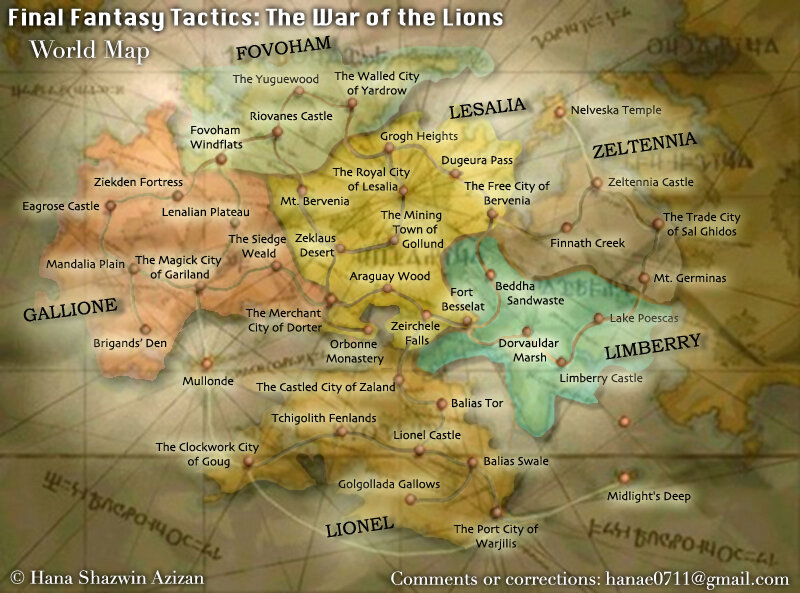
\includegraphics[width=\textwidth]{./art/worldbook/map.jpg}} 	
%
\vspace*{\fill}
%
\accf{\large Fovoham} is a territory in the northernmost part of Ivalice. 
Ruled by Grand Duke Rudolph Barrington, it is separated from the military nation of Romanda by the Rhana Strait. 
Fovoham played an important role in deterring the Romandan invasion in the Fifty Years' War, thanks to the Grand Duke and his assassin squad Khamja. Nowadays, it is the main force behind the Glabados League, and some even say that the Royal Regent, Paul Heiral, is nothing more than a puppet for the
Grand Duke.
\accf{Riovanes Castle} is the home and stronghold of Grand Duke Barrington. 
This castle is distinguished by its Romandan-style towers.
Its position enables not only a great defensive position but also control of all the trade that flows through northern Ivalice, as Mt.~Bervenia serves as natural barrier for the movement of goods and armies.
\accf{Walled City of Yardrow}, also known as Yardrow Fort City is located east of Riovanes Castle and north of the Royal City of Lesalia. It is a fortress city with some ten centuries of history, protected by thick stone walls built to repel invaders. 
This walled city has an important past by securing the northern reaches of Fovoham and presenting an important threat to attacks from the Rhana Strait. 
For centuries, the royal family entrusted this city only to their most loyal vassals, as it is also a prime location for a sneak attack against the capital.
%
\newpage
%
\vspace*{\fill}
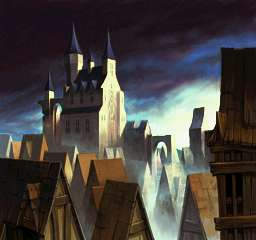
\includegraphics[width=\columnwidth]{./art/worldbook/riovanes.jpg}
%
\vfill
\ofquote{"Our nation exists because of the people! We exist because of them."}{Cidolfus Orlandu}
%
\clearpage
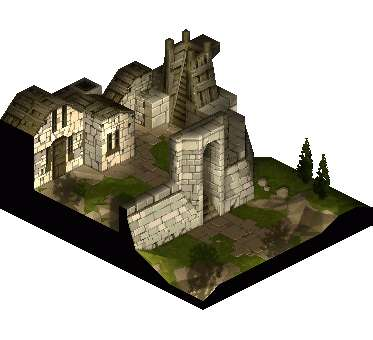
\includegraphics[width=\columnwidth]{./art/worldbook/yardrow.jpg}
\vfill
%
\accf{The Yuguewood}, also known as Yuguo Woods, is located east of Riovanes Castle.
Two-century old yugue trees still grow here, but even this primeval forest was not spared from the ravages of war. 
Albeit the forest may be a great source of building materials, rumors of ghosts haunting its ancient trees keep anyone except for the most courageous or stupid lumberjacks from using it.
\accf{The Fovoham Windflats}, also known as Fovoham Plains, is located east of Ziekden Fortress, and is the location of the Windflat Mill, also known as Windmill Hut. 
These sprawling flatlands are covered by low grasses and battered by fierce winds from the Rhana Straight. 
They are the main farmland area of the Grand Duchy, and provide food not only for Riovanes Castle, but also to Igros Castle as well.
%
\vfill
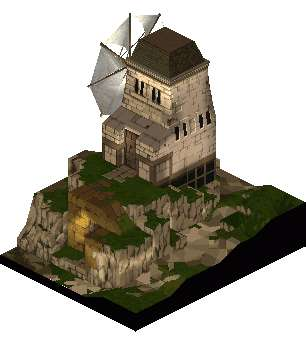
\includegraphics[width=\columnwidth]{./art/worldbook/fovohamplains.jpg}
\newpage
%
\accf{\large Gallionne} is a duchy in the kingdom of Ivalice. 
Ruled by Duke Lestrad Larg, it is located in western Ivalice. 
Its borders are the sea to the west and south, Fovoham to the northeast and Lesalia to the east.
Its seat of power is Eagrose Castle. 
As such, it was held by the Order of the Northern Sky knights during the War of the Lions. 
Lestrad is a stalwart ally of the Grand Duke Barrington, and stands for the Glabados League in the upcoming war.
%
\vfill
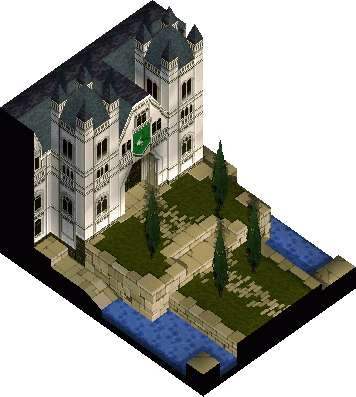
\includegraphics[width=\columnwidth]{./art/worldbook/belouveresidence.jpg}
\vfill
%
\accf{Eagrose Castle}, also known as Igros Castle, is the high seat of Gallionne and home to Duke Larg, its lord. 
This city is second in size only to the royal city of Lesalia. 
During the Lion War, it was the home base of House Beoulve and the Order of the Northern Sky.
It is also the site where the Lucavi demon Adrammelech was defeated.
\accf{The Magick City of Gariland}, also known as Magic City Gariland, is Home to the Royal Academy for the Magickal arts, famous for producing Elidibus, a mage hero of the Fifty Years' War. 
It is located east of Eagrose Castle and west of the Merchant City of Dorter. 
During the Lion War, it was controlled by the Order of the Northern Sky and it contains the academy where Ramza Beoulve and Delita Heiral trained.
\accf{The Merchant City of Dorter}, also known as Dorter Trade City, is a city that developed as a hub for overland trade. 
It is a lively place frequented by all sorts of merchants. 
Located east of the Magick City of Gariland and north of Orbonne Monastery, it sits at a major crossroad in Ivalice. 
It is also home to the biggest congregation of Ajoran faithfuls in Gallionne, and a major opponent to Glabados' influence inside Gallionne.
%
\newpage
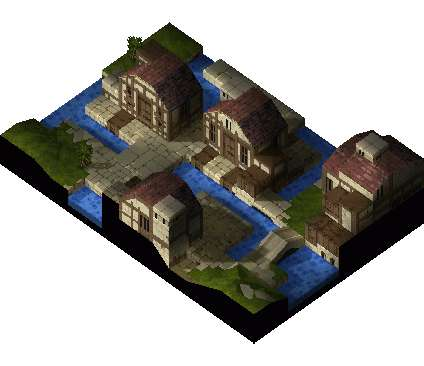
\includegraphics[width=\columnwidth]{./art/worldbook/gariland.jpg}
\vfill
%
\accf{Ziekden Fortress}, also known as Fort Zeakden, is a fortress built during the Fifty Years' War to prevent a Romandan invasion from across the Rhana Strait. 
It is located east of Eagrose Castle. 
Nowadays, it is mostly undefended, as there are few hostilities between Romanda and Ivalice, but should it fall to anyone hostile to Gallionne or Fovoham, it may become an important stronghold.
\accf{The Brigands' Den}, also known as Thieves' Fort, is a small structure built upon a pier, just south of Eagrose Castle. 
Once a refuge for fishermen, it was, for a time, a home to brigands: the chaos that followed the Fifty Year's War turned it into a notorious hideout for thieves, and the Corpse Brigade used it as its stronghold. 
After the War of Lions ended, it was again occupied by fishermen and is part of an important route to Mullonde.
\accf{Mandalia Plains} is a location, famous for its large limestone spires protruding from the ground like the fangs of a great beast.
%
\vfill
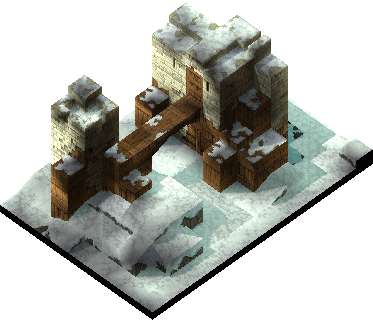
\includegraphics[width=\columnwidth]{./art/worldbook/zeakden.jpg}
\newpage
%
Its white limestone looks like tusks, giving it the name "Beast Plains". 
It is located southeast of Eagrose Castle and west of the Merchant City of Dorter.
\accf{The Siedge Weald}, also known as Sweegy Woods, is an ancient forest surrounded on all sides by mountains. 
Rumors say that it has once been inhabited by Moogles. 
It is located east of the Magick City of Gariland and west of the Merchant City of Dorter.
\accf{Lenalian Plateau}, also known as Lenalia Plateau, is a barren plateau dotted with jagged boulders, but little flora of which to speak.
It is located north of the Magick City of Gariland and south of the Fovoham Windflats.
As it connects the heart of the Gallionne territory with Fovoham, it is part of the main trade routes that connect Dorter to northern Ivalice.
%
\ofpar
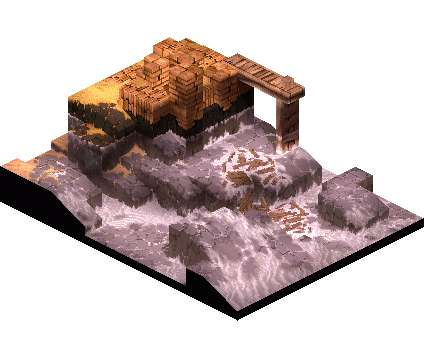
\includegraphics[width=\columnwidth]{./art/worldbook/poeskas.jpg}
\ofpar
%
\accf{\large Limberry} is the easternmost region in Ivalice, ruled by Marquis Henry Elmdore, the young grandson of Messam Elmdore, one of the heroes of the Fifty Years' War who defended the borders of Ivalice from Romandan invaders.
\accf{Limberry Castle} is the stronghold of the Elmdore family, a beautiful white castle that rests on the shores of Loch Dolla. 
Henry Elmdore, who experienced less than twenty winters, rules the land with the passion and the religious fervor only the very young can muster.
His father invited Nox himself as his advisor in his court, and was the first ruler to embrace the Ajoran reformation.
Since his father's conversion, their newfound wealth has helped turn Limberry into an economic powerhouse, and the lands that used to be controlled by the church are more productive than ever.
\accf{Dorvauldar Marsh}, also known as Dolbodar Swamp, is a rich marshland in western Limberry.
The Dorvauldar River carries fertile soil from here to the plains. 
It is located between Fort Besselat and Limberry Castle. 
In the last 60 years, there were intense construction efforts, as dams and irrigation channels were built, taming most of the old swamp areas and creating an important farmland area, transforming it into the breadbasket of Limberry.
\accf{Lake Poescas} was once a large body of water, but now is nothing but a dried lakebed covered in white salt.
It is located just east of Limberry Castle, and is haunted by the living dead. 
Like most of the Zeltennia-Limberry frontier, it is a wasteland devoid of much economic or political importance. 
Salt is mined from its outskirts, but the fear of the undead prevents this area to become the main producer of this good.
%
\vfill
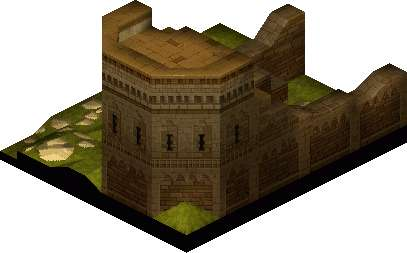
\includegraphics[width=\columnwidth]{./art/worldbook/bethla.jpg}
\vfill
%
\accf{The Beddha Sandwaste}, also known as Bed Desert, is a wild desert covering much of western Limberry, located north of the Order of the Southern Sky fortress of Fort Besselat, and the tombs of ancient emperors can be seen buried in the sand. 
Before the Cataclysm, this used to be an important site of the Holy Empire, but it has transformed from lush farmland to sandy desert almost overnight. 
Caravans travel through it frequently, as it is part of an important trade route, connecting northeastern Ivalice and Lionel.
\accf{Fort Besselat}, also known as Bethla Garrison was the stronghold of the Order of the Southern Sky.
It is located between the Dorvaudar Marsh and the Zeirchele Falls. 
It lies inside the Royal lands of Lesalia, but was taken by a surprise attack by Ajoran forces, and it is under Limberry occupation.
The occupation of Bethla marks the start of the Schism War, and its strategic position oversees most land-based trade routes that pass to Lionel.
%
\vfill
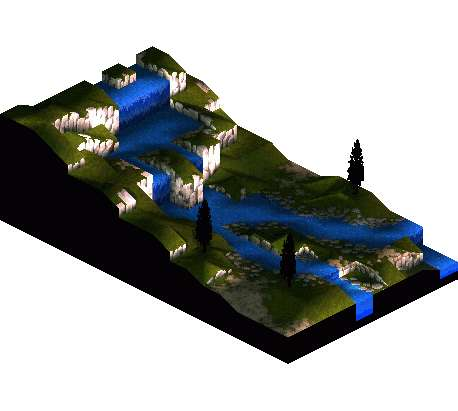
\includegraphics[width=\columnwidth]{./art/worldbook/finath.jpg}
\newpage
%
\accf{\large Zeltennia} is a duchy located in eastern Ivalice, along with the neighboring Limberry.
Zeltennia is ruled by the old Jotan Goltanna, youngest son of Druksmald Goltanna, who fought in the Fifty Years' War and is a descendant of late King Denamda II. 
Straddled at the easternmost border of Ivalice, Zeltennia was known as the fiercest battlefield during the Fifty Years' War. 
It is prone to invasion by the kingdom of Ordallia, and was almost lost to the Ordallian side, if not for the defenses led by Cidolfus Orlandeau, a knight serving House Goltanna.
Nowadays, it sides with Limberry in the Ajoran League.
\accf{Zeltennia Castle} is the stronghold of the Goltanna House.
It was heavily reinforced during the Fifty Years' War, and is now a formidable stronghold.
Goltanna's conversion to the Ajoran faith was born not of faith, but of convenience, as the Zeltennia ruler saw itself surrounded by Ajoran believers both in the south and in the east, and foresaw the potential gains from joining the league and the war that was looming on the horizon.
\accf{Trade City of Sal Ghidos}, also known as Zarghidas Trade City, is hub of trade between Zeltennia and Ordallia. 
Following the events of the Fifty Years' War, it went into decadence, as the sour relations between Ivalice and Ordallia blocked most of the trade. 
However, following the Schism and with the newfound wealth in the Dorvaudar Marsh area, it is experiencing a renaissance, and nowadays it bursts with activity.
%
\ofpar
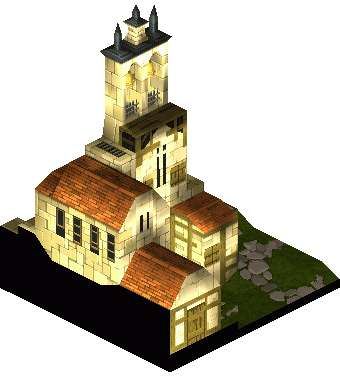
\includegraphics[width=\columnwidth]{./art/worldbook/zeltenniachapel.jpg}
\ofpar
%
\accf{The Finnath Creek}, also known as Finath River, is located between the Free City of Bervenia and Zeltennia Castle. 
It is an important defensive feature, blocking the advance of armies that could launch an attack from the Free City of Bervenia.
Knowing that, Goltanna has positioned most of his armies in a defensive stand in the riverbanks, unsure if he should trespass the imperial land - a hesitation that has not gone unnoticed by his allies.
\accf{Mount Germinas}, also known as Germinas Peak is in the far east of Ivalice. It marks the highest point of a mountain range that dot
the eastern border of both Zeltennia and Limberry, directing most trade to the nearby Sal Ghidos City. 
Its frozen peaks are the source of most of the rivers that once filled up Lake Poescas, but now direct their course westward to the Finath River.
%
\ofpar
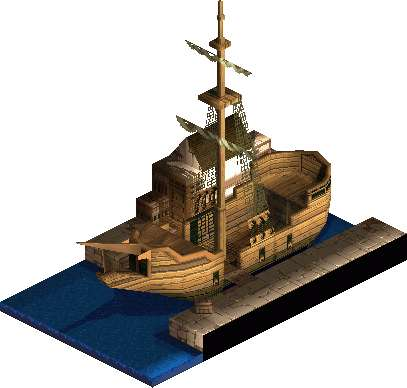
\includegraphics[width=\columnwidth]{./art/worldbook/warjilis.jpg}
\ofpar
%
\accf{\large Lionel} is one of the seven territories of Ivalice. 
It was once known as the land of the Holy Ydoran Empire and the center of the ancient teachings known as Pharism.
Both crumbled after a catastrophe struck the capital, which occurred soon after the execution of Saint Ajora Glabados, who is the central figure in the Glabados and Ajoran faiths. 
Before the Lion War, Lionel continued its role as a religious territory, ruled by Cardinal Delacroix, a prominent figure in the Church and one of the heroes of the Fifty Years' War. 
After the War, with the debacle of the Glabados power, Lionel was reformed into a secular duchy, granted to the Lenande family by the Heiral kings.
\accf{Lionel Castle} is located in Southern Ivalice, and is the stronghold of Leonard Lenande, duke of Lionel. 
It is also the site of Saint Ajora Glabados's capture and of Ramza Beoulve's battle with Cúchulainn. 
Lionel is currently neutral in the Schism War, and emissaries from both the Glabados and the Ajoran leagues try their best to persuade the duke to join the fight.
\accf{The Castled City of Zaland} also known as Zaland Fort City, is an elevated city built atop a low mountain, and serves as a gateway to the province of Lionel. 
It is located in the only land connection between Lionel and mainland Ivalice, and its strategic importance to the whole duchy is paramount.
\accf{The Port City of Warjilis}, also known as Warjilis Trade City, is located south of Lionel Castle along the coast.
As the only merchant city in Lionel, this city developed as a port of transit for trade on the Bugross Sea. 
Warjjilis is an important harbor not only for Lionel, but also for the entire Ivalice kingdom, and the Lionel fleet stationed there is the undisputed strongest naval fleet in the entire region.
\accf{The Clockwork City of Goug}, also known as Goug Machine City, is a mining city located in southwestern Lionel. 
It produces mechanical weapons with generation-old technology.
It is said that the ruins of a lost civilization lie buried beneath the streets of Goug, relics from the age of Saint Ajora, when airships numerous beyond counting filled the skies, and men of iron walked city streets. 
But the art of crafting such things was lost, if it ever truly existed at all.
\accf{The Golgollada Gallows}, also known as the Golgorand Execution Site, is the site of Saint Ajora Glabados's execution. 
It is located south of Lionel Castle and is employed as a public execution ground by the province.
\accf{Tchigolith Fenlands}, also known as Zigolis Swamp, is located west of Lionel Castle and east of the Clockwork City of Goug.
Countless people died here during the Fifty Years' War, changing this once fertile plain into a poisonous fen. 
Even now, more than a century after that war, the scars will not heal, and rumors that some unholy magic was unleashed there run among the common folk.
%
\vfill
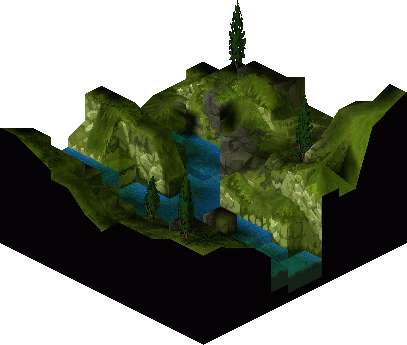
\includegraphics[width=\columnwidth]{./art/worldbook/bariaus.jpg}
\vfill
%
\accf{Balias Tor}, also known as Bariaus Hill, is located north of Lionel Castle. 
It was here that the Holy Ydoran Empire put Balias, the first of Saint Ajora’s disciples, to death. 
It is a holy place for both the Glabados and the Ajoran faithful.
\accf{Balias Swale}, also known as Bariaus Valley, is located between Lionel Castle and the Port City of Warjilis, and is the barren valley where Balias, the first of Saint Ajora's disciples, hid from pursuers from the Holy Ydoran Empire.
\accf{Mullonde Cathedral}, also known as St.~Murond Temple, is the main center of the Glabados Church, and sits on an island to the west of the Lionel mainland. 
Once an independent archbishopric, Mullonde was incorporated into the Lionel Duchy after the Lion War, but remains under the Church's control.
%
%
\clearpage
%
\accf{\large Lesalia} is the center of the kingdom of Ivalice in Final Fantasy Tactics. 
It was the seat of the Atkascha royal family, who have ruled from this region even during the Fifty Years' War and the War of the Lions, but now houses the Heiral royal family. 
The signs of wealth and luxury persisted even as Ivalice faced war after war.
\accf{The Royal City of Lesalia}, also known as Lesalia Imperial Capital is the capital of the kingdom Ivalice. 
It is the high seat of the Crown, and in it towers the luxurious keep that houses Ivalice's royal family. 
As the king is comatose and Paul Heiral, the regent, dances by the music played by the Fovoham Grand Duke, the royal lands are aligned with the Glabados league, but the Regent's inability to coordinate his armies has led to many early Ajoran victories. 
If he can join forces with the main Glabados armies, the tides of this war may turn.
\accf{The Mining Town of Gollund}, also known as Goland Coal City, is located south of the Royal City of Lesalia and contains a large coalmine. 
Rich in mineral resources, these highlands where the town lies are also battered by year-round snowstorms.
\accf{The Bervenia Free City}, famous for being Saint Ajora Glabados's birthplace, is under the direct control of the Church of Glabados.
It is located on the road between the Royal City of Lesalia and Zeltennia Castle. 
It is the most direct course from Zeltennia to the capital, but it was not attacked until now.
%
\ofpar
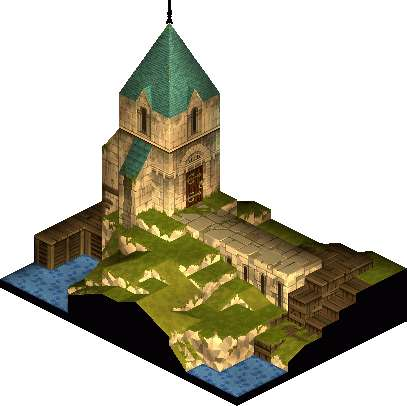
\includegraphics[width=\columnwidth]{./art/worldbook/orbonne.jpg}
\ofpar
%
\accf{Orbonne Monastery} was built more than twelve centuries ago, and is under the control of the Church of Glabados. 
It houses the Underground Book Storage, a mysterious library holding old tomes from the era of St.~Ajora. 
It is said to be filled with many great literary works, such has historical writings and scriptures including works in foreign languages. 
The literary works are strewn in piles of disarray on the floors, and ancient scrolls and lithographs are piled among the printed works. 
Priests are restricted in going to the third underground floor. 
In the deepest area of the vault, the floor covers a tunnel entrance, and a magical rune is inscribed on the floor.
\accf{The Zeklaus Desert} lies north of the Merchant City of Dorter on the road to the Royal City of Lesalia, and is the location of the Sand Rat Sietch, where Marquis Elmdore was held hostage by the Corpse Brigade. 
Scorching in the daytime and freezing at night, it is no mystery why so few travel through this desert. Because of that, most of the trade that goes to Lesalia uses Fovoham as a route, instead of going through the most direct route by Dorter.
%
\vfill
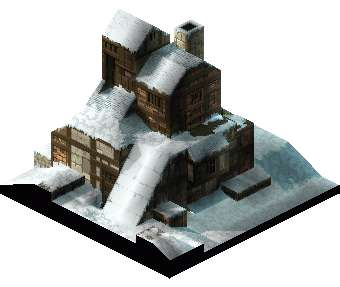
\includegraphics[width=\columnwidth]{./art/worldbook/goland.jpg}
\vfill
%
\accf{Mount Bervenia}, also known as Bervenia Volcano is the largest active volcano in Ivalice and located southeast of Riovanes Castle. Molten lava flows down its surface, white ash and smoke darken the sky. 
It is the second reason Zeklaus is not used as a trade route, except for smugglers and the most daring of merchants.
\accf{Araguay Woods} is located east of the Merchant City of Dorter and is a sprawling forest covering the southern Lesalian region inhabited by a variety of rare fauna. 
Its wood is famous in all Ivalice, and much of it adorns the richest castles in the kingdom.
\accf{Grogh Heights}, also known as Grog Hill, is located between the Royal City of Lesalia and the Walled City of Yardrow. 
The heights compose the largest farm belt in the Lesalia region, and most of the crops harvested here are destined for the capital city. 
It is one of the oldest and most developed farmland regions of the entire kingdom.
\accf{Zeirchele Falls}, also known as Zirekile Falls is a great waterfall located west of Fort Besselat. Few can help but be enchanted by the sight of Zeirchele Falls cascading down the stair like Algost Mountains. 
The waters of the falls go eastward to Limberry, to feed the riches of Dorvaudar.
\accf{Dugeura Pass}, also known as Dogoula Pass, is located on the road between Riovanes Castle and Zeltennia Castle. 
Nearly 2,000 dohms in height, Mount Landria was once used by monks as a holy place of fasting and atonement. 
This passage is the safest route between the Grogh region and Bervenia, and even a small force could defend it from an attack, should the need arise.
%
%
\clearpage
%
\ofsubsubsection{Campaign Ideas}
%
\onecolumn
%
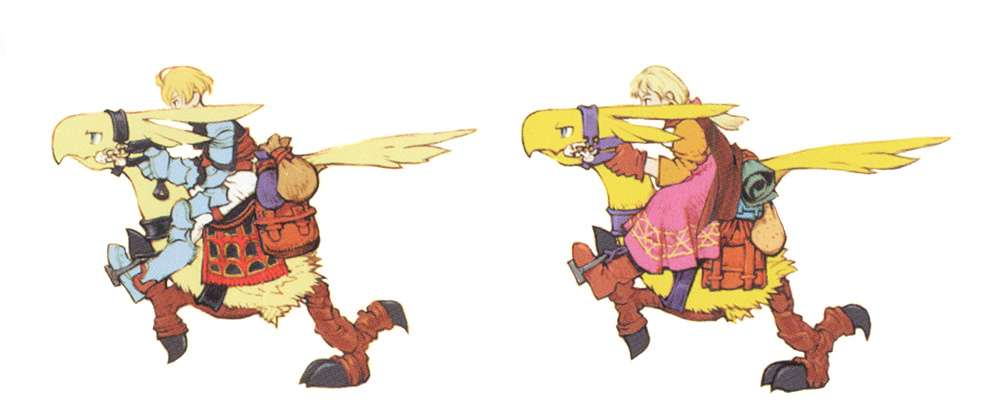
\includegraphics[width=\textwidth]{./art/worldbook/chocobos.jpg}
%
\vfill
%
\begin{multicols}{2}
%
\accf{Campaign Idea - Mythological Heroes:}
Set in the Age of Myths, the players will explore the tales of the legendary heroes of Baron, Paramecia, Kushuka and Melmond. This age is akin to more
traditional Final Fantasy histories, as it includes guns, magic and magitek, airships, flying continents, non-humans, and a general high-fantasy theme.
Adventure hooks include the wars between the kingdoms, the discovery of the Ronan ruins and artifacts, the Kashuka revolution and the fight of the first Zodiac Braves against Lucavi and his demons.
%
\ofpar
%
\accf{Campaign Idea - Ydoran Intrigue:}
The Holy Ydoran empire was a very busy place. 
Nobles and courtly intrigue abound, and while it still had the high levels of technology and magic of the previous era, the strict social order and iron fist enforced by the Ydoran rulers on their quick conquest makes this a prime candidate for espionage and social drama.
Along with that, the five decades before the Cataclysm also saw the rise of St Ajora, who himself was also a Ydoran spy.
Lots of religious conflict with the Pharism vs Ajora debate, along with the second Lucavi plot make this an exciting setting for adventures.
%
\ofpar
%
\accf{Campaign Idea - The Cataclysm:}
Starting with the execution of St.~Ajora, this campaign explores the events around the time of the Cataclysm.
Therefore, the story can give insight into the height and sudden destruction of one of the most advanced civilizations in the history of Ivalice.
The players take the role of heroes who fight alongside the hero-king Mesa to save humanity and possibly also other races of Ivalice from the effects of the Cataclysm.
In this foray into the supernatural, they have to face divine champions and catastrophes and maybe even the gods themselves.\\
%
\columnbreak\\
%
\accf{Campaign Idea - Warring Kingdoms:}
Set in between the first and fifth centuries after the Cataclysm, this campaign hook explores the conflicts between the six kingdoms of Kaladis and the rise to prominence of Mullonde and the Glabados Church.
In this moment of time, Lesalia, Fovoham, Zeltennia, Gallionne, Lionel and Limberry were independent kingdoms, forging aliances and warring constantly between themselves. 
Unlike the earlier eras, there are no more non-humans and high magic, with the technology level regressing to a level comparable to the early periods of the middle ages.
%
\ofpar
%
\accf{Campaign Idea - Wars of Ivalice:}
This campaign idea is set in the sixty years between the two last major wars Ivalice has undergone: the Fifty Year’s war and the War of the Lions.
This period can be visited either to recreate the events of the videogame by another point of view, or to explore untold tales of unsung heroes from either side of the conflict.
How was life inside Romanda and what is the aftermath of its defeat? 
What voices inside the Church begged for reason before they started to plot the Lion War?
How did the common folk react after the fall of the Corpse Brigade? 
These questions can warrant interesting stories to be told.
%
\ofpar
%
\accf{Campaign Idea - The Schism:}
This is the default setting for this worldbook, set in 1250 A.C.
The schism between the Ajoran and Glabados faiths sparks the underlying tensions of the kingdom, leading to the formation of the two religious leagues. 
Which side will the players take in this conflict? 
How will the other nations respond to Ivalice’s weaknesses? 
What are the secret motives of the major political players?
%
\end{multicols}
%
\vfill
%
\hspace*{\fill}\ofquote{"A small stone may only make a small ripple at first, but someday it will be a wave."}{Wiegraf Folles}\hspace*{\fill}\\
%
\twocolumn
\clearpage
%
\ofsubsubsection{Optional Rules}
%
The following is a collection of optional rules and content, which you can use to create a closer feeling to Final Fantasy Tactics.
%
\vfill
%
\accf{Grid-based Combat:}
You can use a square grid to visualize combat in the same manner as FFT.
Each square is 1u by 1u in size and player characters take up 1 square of space.
The distance between two squares is the sum of the horizontal and vertical squares between them, this system is called the \accf{Manhattan~distance}.
In other words, adjacent squares to your up, down left and right have a distance of 1u from you, but adjacent diagonal ones have a distance of 2u.
Ranges and target distances for abilities are adjusted accordingly.
The example below shows the normal (2u) target shape, as well as the special shapes line (5u) and front (2u). 
The blue squares represent the caster, while the red ones represent enemy combatants.
%
\vfill
%
\begin{figure}[h!]
	\centering
	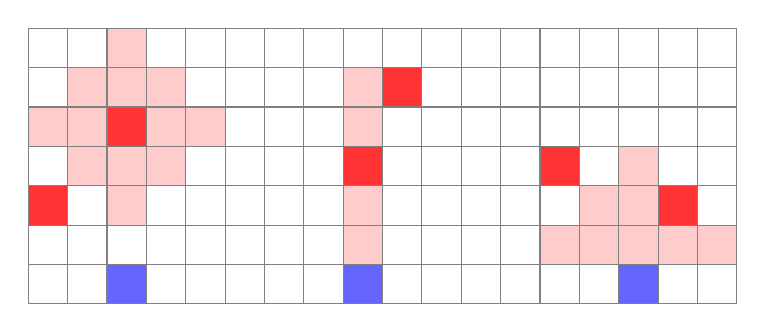
\begin{tikzpicture}[]
	\tikzstyle{filled}=[draw, black!50!white, rectangle, thin, minimum height = 0.5cm, minimum width=0.5cm]
	\tikzstyle{target}=[fill=red!20!white]
	\tikzstyle{caster}=[fill=blue!60!white]
	\tikzstyle{enemy}=[fill=red!80!white]	
	\draw[step=0.5,black!50!white, thin,xshift=-0.25cm,yshift=-0.25cm] (0,0) grid (9, 3.5);	
	%Normal
	\node[filled, caster](g0)at (1, 0) {};
	\node[filled, enemy](g0)at (1, 2) {};
	\node[filled, enemy](g0)at (0, 1) {};
	\node[filled, target](g0)at (1, 1) {};
	\node[filled, target](g0)at (1, 1.5) {};
	\node[filled, target](g0)at (1, 2.5) {};
	\node[filled, target](g0)at (1, 3) {};
	\node[filled, target](g0)at (1.5, 2.5) {};
	\node[filled, target](g0)at (0.5, 2.5) {};
	\node[filled, target](g0)at (1.5, 1.5) {};
	\node[filled, target](g0)at (0.5, 1.5) {};
	\node[filled, target](g0)at (1.5, 2) {};
	\node[filled, target](g0)at (2, 2) {};
	\node[filled, target](g0)at (0, 2) {};
	\node[filled, target](g0)at (0.5, 2) {};
	%Line
	\node[filled, caster](g0)at (4, 0) {};
	\node[filled, enemy](g0)at (4, 1.5) {};
	\node[filled, enemy](g0)at (4.5, 2.5) {};
	\node[filled, target](g0)at (4, 0.5) {};
	\node[filled, target](g0)at (4, 1) {};
	\node[filled, target](g0)at (4, 2) {};
	\node[filled, target](g0)at (4, 2.5) {};	
	%Front
	\node[filled, caster](g0)at (7.5, 0) {};
	\node[filled, enemy](g0)at (8, 1) {};
	\node[filled, enemy](g0)at (6.5, 1.5) {};	
	\node[filled, target](g0)at (7.5, 0.5) {};
	\node[filled, target](g0)at (7.5, 1) {};
	\node[filled, target](g0)at (7.5, 1.5) {};
	\node[filled, target](g0)at (8, 0.5) {};
	\node[filled, target](g0)at (8.5, 0.5) {};
	\node[filled, target](g0)at (7, 0.5) {};
	\node[filled, target](g0)at (6.5, 0.5) {};
	\node[filled, target](g0)at (7, 1) {};
	\end{tikzpicture}
\end{figure}
%
\vfill
%
\accf{Directional Defense:}
In conjunction with a square grid, you can also change the potency of a combatant's defense depending on the direction they are attacked from.
At the end of every turn, combatants have to announce the direction that they are facing. 
There are 4 possible directions (up, down, left and right), so the one they are facing is their front, the opposite direction is their back and the two remaining directions are their sides. 
Whenever combatants are Attacked from a side, their DEF is halved when calculating the suffered damage.
Whenever combatants are Attacked from behind, their Evasion DC is increased by 2 while trying to evade the Attack.
%
\vfill
%
\accf{Monsters of Ivalice:}
Below are examples of monsters that are common in the world of Ivalice.
Apart from these, the following monsters from the bestiary supplement may also be encountered:
Skeleton, Ghoul, Cockatrice, Ahriman, Coeurl, Mindflayer, Malboro, Behemoth, Red Dragon.
%
\vfill
%
\ofmonster{Floating Eye}{4}{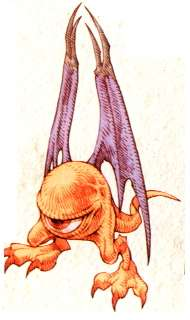
\includegraphics[width=0.16\columnwidth]{./art/worldbook/eye.jpg}}
{
	HP: & \hfill 32 & MP: & \hfill 30 \\
	STR: & \hfill 2 & DEF: & \hfill 2 \\
	MAG: & \hfill 5 & RES: & \hfill 4 \\
	AGI: & \hfill 4 & Size: & \hfill S\\
}
{\accf{Beam}: 2d DMG, 3u Range \hfill \accf{Immune:}\sleep\silence\blind}
{	
	\mtech{Wing Buffet}{5}{0r}{3u (front)}{Self}{Enemies in the target area suffer 2d wind damage.}{}
}
%
\newpage
%
\ofmonster{Goblin}{2}{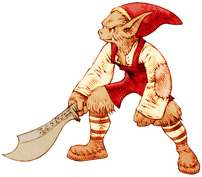
\includegraphics[width=0.26\columnwidth]{./art/worldbook/goblin.jpg}}
{
	HP: & \hfill 16 & MP: & \hfill 18\\
	STR: & \hfill 2 & DEF: & \hfill 1 \\
	MAG: & \hfill 0 & RES: & \hfill 0 \\
	AGI: & \hfill 3 & Size: & \hfill M\\
}
{\accf{Knife}: 1d DMG \hfill \accf{Immune:}\poison\immobile}
{
	\mtech{Goblin Punch}{2}{0r}{Single}{Weapon}{Make an Attack against the target. If you hit, you push him back by 1u on top of the damage dealt.}{}		
	\mtech{Spin Punch}{4}{0r}{1u}{Self}{Make an Attack against everyone within 1u.}{}		
}
%
\vfill
%
\ofmonster{Red Chocobo}{3}{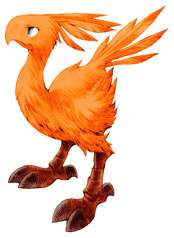
\includegraphics[width=0.18\columnwidth]{./art/worldbook/chocobo-red.jpg}}
{
	HP: & \hfill 28 & MP: & \hfill 16\\
	STR: & \hfill 3 & DEF: & \hfill 2 \\
	MAG: & \hfill 1 & RES: & \hfill 1 \\
	AGI: & \hfill 4 & Size: & \hfill M\\
}
{\accf{Beak}: 1d DMG \hfill \accf{Resilient}:\fire}
{	
	\mtech{Choco Kick}{4}{0r}{Single}{Weapon}{The target suffers 3d damage and is knocked back by 1u.}{}
	\mreaction{Choco Counter}{Whenever you are hit by an Attack, immediately makean Attack on the perpetrator.}
}
%
\vfill
%
\ofmonster{Grenade}{4}{
\includegraphics[width=0.22\columnwidth]{./art/worldbook/bomb.jpg}}
{
	HP: & \hfill 35 & MP: & \hfill 20\\
	STR: & \hfill 2 & DEF: & \hfill 2 \\
	MAG: & \hfill 0 & RES: & \hfill 1 \\
	AGI: & \hfill 3 & Size: & \hfill M\\
}
{
	\accf{Tackle}: 2d DMG \hfill \accf{Resilient}:\fire \hfill \accf{Weak}:\ice\water
}
{
	\mtech{Flame Attack}{5}{0r}{Single}{2u}{The target suffers 3d fire damage.}{\fire}		
	\mtech{Self-Destruct}{0}{1r}{2u}{Self}{Inflict KO on yourself to deal 6d fire damage to everyone within the target area.}{\fire}		
}
%
\vfill
%
\ofmonster{Revenant}{5}{
\includegraphics[width=0.2\columnwidth]{./art/worldbook/ghost.jpg}}
{
	HP: & \hfill 50 & MP: & \hfill 40\\
	STR: & \hfill 3 & DEF: & \hfill 3 \\
	MAG: & \hfill 5 & RES: & \hfill 6 \\
	AGI: & \hfill 2 & Size: & \hfill M\\
}
{
	\accf{Touch}: 2d DMG \hfill \accf{Weak}:\holy \hfill \accf{Immune:}\poison\immobile\sleep
}
{
	\mtech{Zombie Touch}{4}{0r}{Single}{Weapon}{Make an Attack against the target. If you hit, he suffers Zombie for 10 rounds on top of the damage dealt.}{}	
	\mtech{Drain Touch}{5}{0r}{Single}{Weapon}{Make an Attack against the target. If you hit, increase your HP by 1d on top of the damage dealt.}{}	
}
%
\clearpage
%
\accf{Bravery \& Faith:} 
To create more heroic moments in your adventure, you can allow characters to derive special powers from their Bravery or Faith.
Every character tracks one resource pool for each, that can hold up to 5 points.
Players roll 1d for each during character creation to determine their starting Bravery and Faith (a 6 is rounded down to a 5).
Characters recover 1 point of Bravery and 1 point of Faith whenever they go to sleep and they can never spend more than 1 point of either at once.
\accf{Bravery} allows characters to channel their inner courage to reach beyond their usual abilities.
Characters can spend 1 point of Bravery whenever they perform a check to add 1 to the result of their roll.
They can also spend 1 point of Bravery whenever they deal any damage during combat to add 1d to the total damage dealt.
When a character's Bravery drops to 0, all of their total damage dealt is halved.
The GM can award additional points of Bravery whenever someone acts particularly heroic or deduct a point when they act cowardly.
\accf{Faith} helps characters to overcome failures through confidence in their beliefs.
Characters can spend 1 point of Faith whenever they perform a check to re-roll one die after seeing the result.
They can also spend 1 point of Faith whenever they suffer any damage during combat to reduce the total damage suffered by 1d.
The GM can award additional points of Faith whenever someone acts in accordance to their belief system and deduct a point when they act against it.
When a character's Faith drops to 0, they have Disadvantage on every check that they perform.
%
\vfill
%
\ofquote{"Most people have to act the roles given to them. Then again, most of them haven't even noticed they're acting."}{Delita Hyral}
%
\vfill
%
\accf{Hiring Soldiers:} 
In the world of Ivalice, many capable combatants will offer their services for the right price.
As such, the party can hire paid soldiers in almost any major city to improve their combat strength.
These soldiers are controlled by the GM during battles and generally should not play a major role outside of it.
Accordingly, you also do not need to track their current experience and progression. 
For characters of greater importance, we recommend to use the standard character creation rules, if necessary you
can convert a hired soldier to a fully fledged character later on.
When using the \accf{Bravery \& Faith} rules, a hired soldier will immediately leave the party when either their Bravery or Faith drops to 0.
On the right are some examples of soldiers that can be hired, along with their required daily salary.
As these are very common types of combatants, you can also use them as human enemies.
%
%
%
\newpage
%
\ofmonster{Squire}{1}{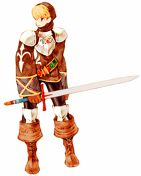
\includegraphics[width=0.22\columnwidth]{./art/worldbook/squire-male.jpg}}
{
	HP: & \hfill 15 & MP: & \hfill 12\\
	STR: & \hfill 2 & DEF: & \hfill 1 \\
	MAG: & \hfill 0 & RES: & \hfill 0 \\
	AGI: & \hfill 3 & Size: & \hfill M\\
}
{\accf{Sword}: 1d DMG \hfill \accf{Salary:} 25G per day}
{
	\mtech{Throw Stone}{2}{0r}{Single}{3u}{The target suffers 1d damage.}{}
	\ofrow\accf{Items:} 1x Potion		
}
%
\vfill
%
\ofmonster{Chemist}{2}{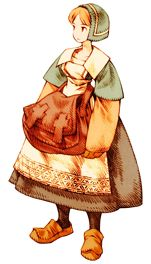
\includegraphics[width=0.14\columnwidth]{./art/worldbook/chemist-female.jpg}}
{
	HP: & \hfill 2 & MP: & \hfill 26\\
	STR: & \hfill 1 & DEF: & \hfill 1 \\
	MAG: & \hfill 1 & RES: & \hfill 1 \\
	AGI: & \hfill 2 & Size: & \hfill M\\
}
{\accf{Knife}: 1d DMG \hfill \accf{Salary:} 50G per day}
{
	\mtech{Aid}{4}{0r}{Single}{1u}{Remove one negative Status Effect from the target except KO.}{}	
	\mreaction{Auto-Potion}{Whenever an ally within 1u suffers damage, you can immediately use an Item on them.}		
	\ofrow\accf{Items:} 3x Potion, 1x Phoenix Down, 1x Remedy
}
%
\vfill
%
\ofmonster{Archer}{3}{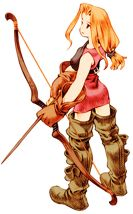
\includegraphics[width=0.16\columnwidth]{./art/worldbook/archer-female.jpg}}
{
	HP: & \hfill 27 & MP: & \hfill 18\\
	STR: & \hfill 1 & DEF: & \hfill 1 \\
	MAG: & \hfill 0 & RES: & \hfill 1 \\
	AGI: & \hfill 2 & Size: & \hfill M\\
}
{\accf{Bow}: 2d DMG, 5u range \hfill \accf{Salary:} 100G per day}
{
	\mtech{Aim}{2}{0r}{Single}{Self}{On the next Attack that you perform, the target has Disadvantage on the evasion check.}{}	
	\ofrow\accf{Items:} 2x Potion, 1x Eyedrops	
}
%
\vfill
%
\ofmonster{Knight}{4}{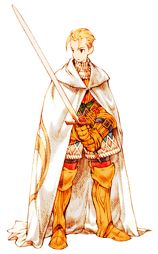
\includegraphics[width=0.17\columnwidth]{./art/worldbook/knight-male.jpg}}
{
	HP: & \hfill 38 & MP: & \hfill 25\\
	STR: & \hfill 4 & DEF: & \hfill 2 \\
	MAG: & \hfill 0 & RES: & \hfill 1 \\
	AGI: & \hfill 3 & Size: & \hfill M\\
}
{\accf{Sword}: 2d DMG \hfill \accf{Salary:} 150G per day}
{
	\mtech{Rend Power}{5}{0r}{Single}{Weapon}{
		Make an Attack against the target.  If you hit, the damage dealt is halved and the target suffers DeSTR for 3 rounds.
	}{}	
	\mtech{Rend Magick}{5}{0r}{Single}{Weapon}{
		Make an Attack against the target.  If you hit, the damage dealt is halved and the target suffers DeMAG for 3 rounds.
	}{}	
	\ofrow\accf{Items:} 1x Hi-Potion, 1x Remedy	
}
%
\clearpage